\documentclass[10pt,a4paper]{article}
\usepackage[margin=17mm]{geometry}
\usepackage{graphicx,booktabs,hyperref,xcolor}
\pagestyle{empty}
\begin{document}
\noindent{\Large\bfseries Certified relation pruning and native controls}\\[3pt]
{\small Rust integration and fixed-input diagnostics, 27 November 2026. PR \#5251.}\\[3pt]
{\small p31=$2147483647$; p53=$9007199254740881$. Seed7 LAST-star, $n=3,4,6$.}

\paragraph{Result.} Preserving every closed space at $D=2,3,4$ retained all 4/4, 6/6 and 10/10 candidate rows at $n=3,4,6$ on both declared primes. This specific sparsity lead is negative. All values are unsigned producer evidence; no new PCC ledger claim or execution attestation. [pcc:unverified]
\begin{center}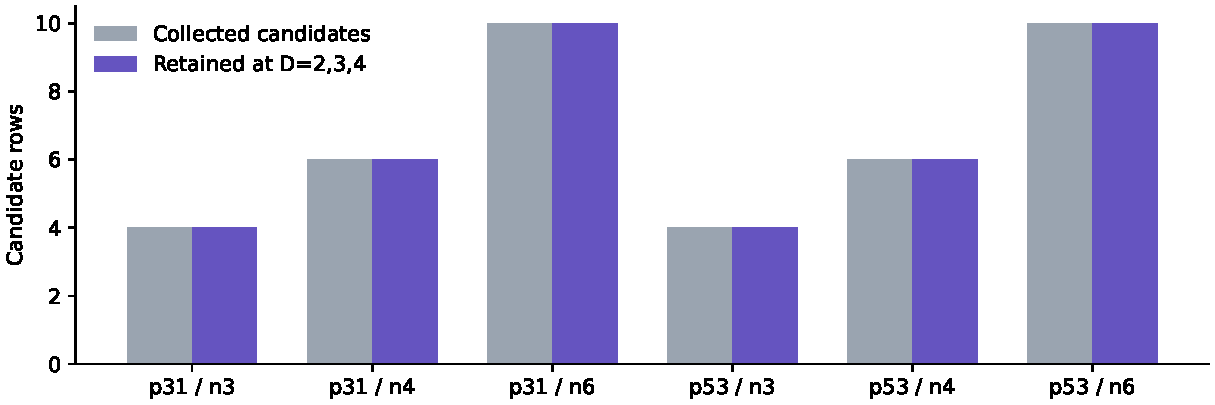
\includegraphics[width=\linewidth]{pruning-retention.pdf}\end{center}
\noindent The sequential algorithm tests each deletion against surviving rows. Rejected deletions stop at a replay-certified obstruction; later skipped caps are uncomputed. Every accepted deletion must preserve every cap and any supplied full $[R|a|b]$ scalar-label span. These polynomial fixtures have no curve/group-row labels. Solving degree and intrinsic regularity remain null.
\paragraph{Native checks.} The opt-in API reuses the existing acyclic product/chain checker. The default API retains exhaustive checking. The same original, proof, basis and replay statistics are required in 108 matched cases spanning all six wire forms, three kernels and six inputs. [pcc:unverified]
\begin{center}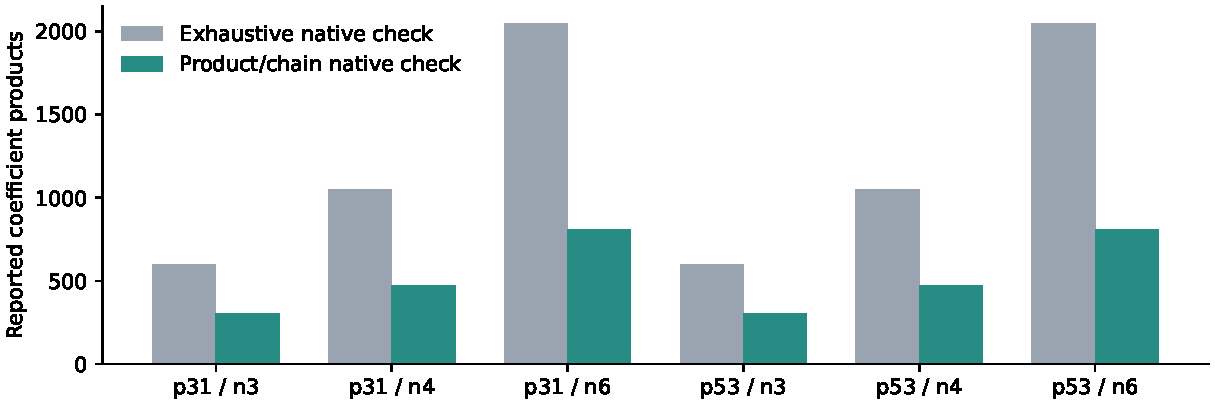
\includegraphics[width=\linewidth]{native-check-products.pdf}\end{center}
\noindent\small Plot: the flat-DAG/batch487 arm only; all 108 paired records are retained. These are reported native-check counters, not independently attested costs or whole-call runtimes. Graph setup and all other phases remain unpriced by this plot. No 15$\times$ speedup is established. [pcc:unverified]
\newpage
\noindent{\Large\bfseries Validation and custody}
\begin{center}\begin{tabular}{ll}\toprule
Scope & Recorded outcome\\\midrule
Producer library &92 tests pass\\
Producer with field counters &93 tests pass\\
Independent checker library &14 tests pass\\
Pruning/control/codec qualifier &12 tests pass\\
Fixed pruning inputs &6 scan/replay cases complete\\
Original root integration &36 cases; 252 mutation refusals\\
Native-check comparison &108 pairs; 864 mutation refusals\\
Separate stored-proof replay &36 plus 108 complete replays\\
Auditor sabotage views &2 original, 5 new refused\\\bottomrule\end{tabular}\end{center}
\noindent All rows above are source-scoped, unsigned correctness results. [pcc:unverified]
\paragraph{Source correction.} Failed Git lazy restores left two empty tracked files. The first helper mistook presence for hydration. One empty panel file was embedded in the library, so earlier canonical-closure wording was too broad. Both preimages, original source pins, workers' hashes and logs are retained. Exact indexed blobs were restored; all 552 tracked literal targets match Git. The root was rebuilt and the 36/108 matrices and separate audits were repeated. Their 181/433 payload files match the prior contexts byte for byte. [pcc:unverified]
\paragraph{Whole root-unit scope.} Whole default-feature root-unit compilation remains unqualified: both bounded attempts failed memory allocation; no full-suite runtime was executed. This is separate from the repaired-source native integration. No unrelated algorithm or test was removed; failures and resource limits remain in the raw logs.
\paragraph{Retained failures.} GitHub comparison/fetch errors, wrapper lock/compiler-path setup errors, the deliberately interrupted first full-cap pruning scan (exit 143), its two completed files and source preimages remain available. The fresh streaming/first-obstruction run uses distinct source, pre-call, output and post-call records.
\paragraph{Measurement limits.} No comparative timing ran. The original full application-call boundary, strongest matched controls, both primes, $n=3,4,6$, seed 7 LAST-star, repeated/A/A design, complete proofs and 15$\times$ acceptance remain. Canonical timing instructions are still VLT1-encrypted. The user's Conductor and checkpoint/S3 waivers do not resolve that separate document dependency.
\paragraph{Reproduction.} See README.md and REPRODUCE.md; source rosters, plans, immutable-worker hashes, reference inputs, raw logs and archives are in this study. Audit results have no independent-host or signed-execution verdict. The report renderer only lays out stored Rust outputs.
\end{document}
